\documentclass[oneside]{scrreprt}

\usepackage[utf8]{inputenc}

\inputencoding{utf8}

\usepackage{blindtext}
\usepackage{graphicx}
\usepackage{abstract}
\usepackage[headsepline]{scrlayer-scrpage}
\usepackage{listings}
\usepackage[hidelinks,bookmarks,urlcolor=uniblue]{hyperref}
\usepackage{mathtools}
%\usepackage{ftnright}
\pagestyle{scrheadings}
\graphicspath{ {./pics/} }
\usepackage{xcolor}
\usepackage{soul}
\usepackage{url}
\usepackage{svg}
\usepackage{amsmath}
\usepackage{xcolor}
\usepackage{doi}
\usepackage{tikz}
\usetikzlibrary{arrows.meta,calc,fadings,backgrounds}
\usepackage{float}
\usepackage{array}

\definecolor{Light}{gray}{.90}
\sethlcolor{Light}

\definecolor{uniblue}{RGB}{0,99,166}
\definecolor{uniwine}{RGB}{246,168,0}
\definecolor{uniwine}{RGB}{167,28,73}
\definecolor{unilightgreen}{RGB}{148,193,84}
\definecolor{unigrey}{RGB}{102,102,102}

\newcommand{\code}[1]{\texttt{\hl{#1}}}

\usepackage[backend=biber,style=chem-acs,bibencoding=utf8]{biblatex}
\DeclareFieldInputHandler{note}{% deletes the unneccessary Publisher/etex entries
  \def\NewValue{}}

\addbibresource{references_zotero.bib}
\title{Implementation of Auxiliary Restraints for Relative Binding Free Energy Calculations in the 'common-core serial-atom-insertion' Framework \texttt{Transformato}}
\author{Supervised by: Univ-Prof. Dr. Stefan Boresch\\Submitted by: \hspace{26mm}Alexander Grasser}
\date{June 2022}
\publishers{Department of Computational Biological Chemistry\\University of Vienna\\
\includegraphics[width=5cm]{Uni_Logo_2016.jpg} }
\subject{Thesis for the title Bachelor of Science in Chemistry}

\automark[chapter]{chapter}
\ihead{Bachelor's Thesis}
\chead{}

\ohead{\headmark}


\RedeclareSectionCommand[pagestyle=scrheadings,beforeskip=0pt]{chapter}






\begin{document}

\begin{titlepage}

\maketitle{}
\end{titlepage}
\section*{Abstract}
    
    For protein-ligand affinity at binding sites, the relative (and absolute) binding free energy is arguably the most important indicator. Traditionally, calculating these energies is done using comprehensive, GPU-assisted "soft-core" modeling. The 'common-core serial-atom-insertion' framework \texttt{Transformato} instead allows to efficiently divide the problem into sequential fragments solvable by traditional MD calculations. However, issues arise when ligands leave the binding site during simulation. This work presents a possible solution by enabling both automatic and manual addition of restraints to the system.
\vspace{\fill}
\section*{Notes}
\noindent\begin{minipage}{0.7\textwidth}
The data compiled for this thesis may be accessed at GitHub under \url{https://github.com/agrass15268/AuxiliaryRestraintsTransformato/tree/data} or with the QR - Code to the right.
\end{minipage}
\hspace{0.1\textwidth}
\begin{minipage}{0.2\textwidth}
\includesvg[height=2cm]{qrcode}
\end{minipage}
 
\vspace{1cm}

\noindent\begin{minipage}{0.7\textwidth}
Source code and packaged versions of the \texttt{Transformato} package may be retrieved from its GitHub repository at  \url{https://github.com/wiederm/transformato} or with the QR - Code to the right.
\end{minipage}
\hspace{0.1\textwidth}
\begin{minipage}{0.2\textwidth}
\includesvg[height=2cm]{qrcodetrafo}
\end{minipage}
\newpage

\begingroup
\let\clearpage\relax
\renewcommand\contentsname{Table of Contents}
\tableofcontents
\addtocontents{toc}{~\hfill\textbf{Page}\par}
\endgroup
%\renewcommand{\thefootnote}{\Roman{footnote}}
\chapter{Introduction}
Almost since the inception of computer-assisted molecular modeling, a significant focus has been on the interaction of pharmaceutically active biomolecules. Designing and testing lead compounds to catalyze or inhibit biochemical processes is a major focus of research and development efforts, and a comparatively easy-to-access parameter with nevertheless good predictive capabilities has long been the relative binding free energy difference, especially with recent advancements in computational power \cite{cournia_relative_2017}.

\begin{figure}[h]
    \begin{center}
        
    
    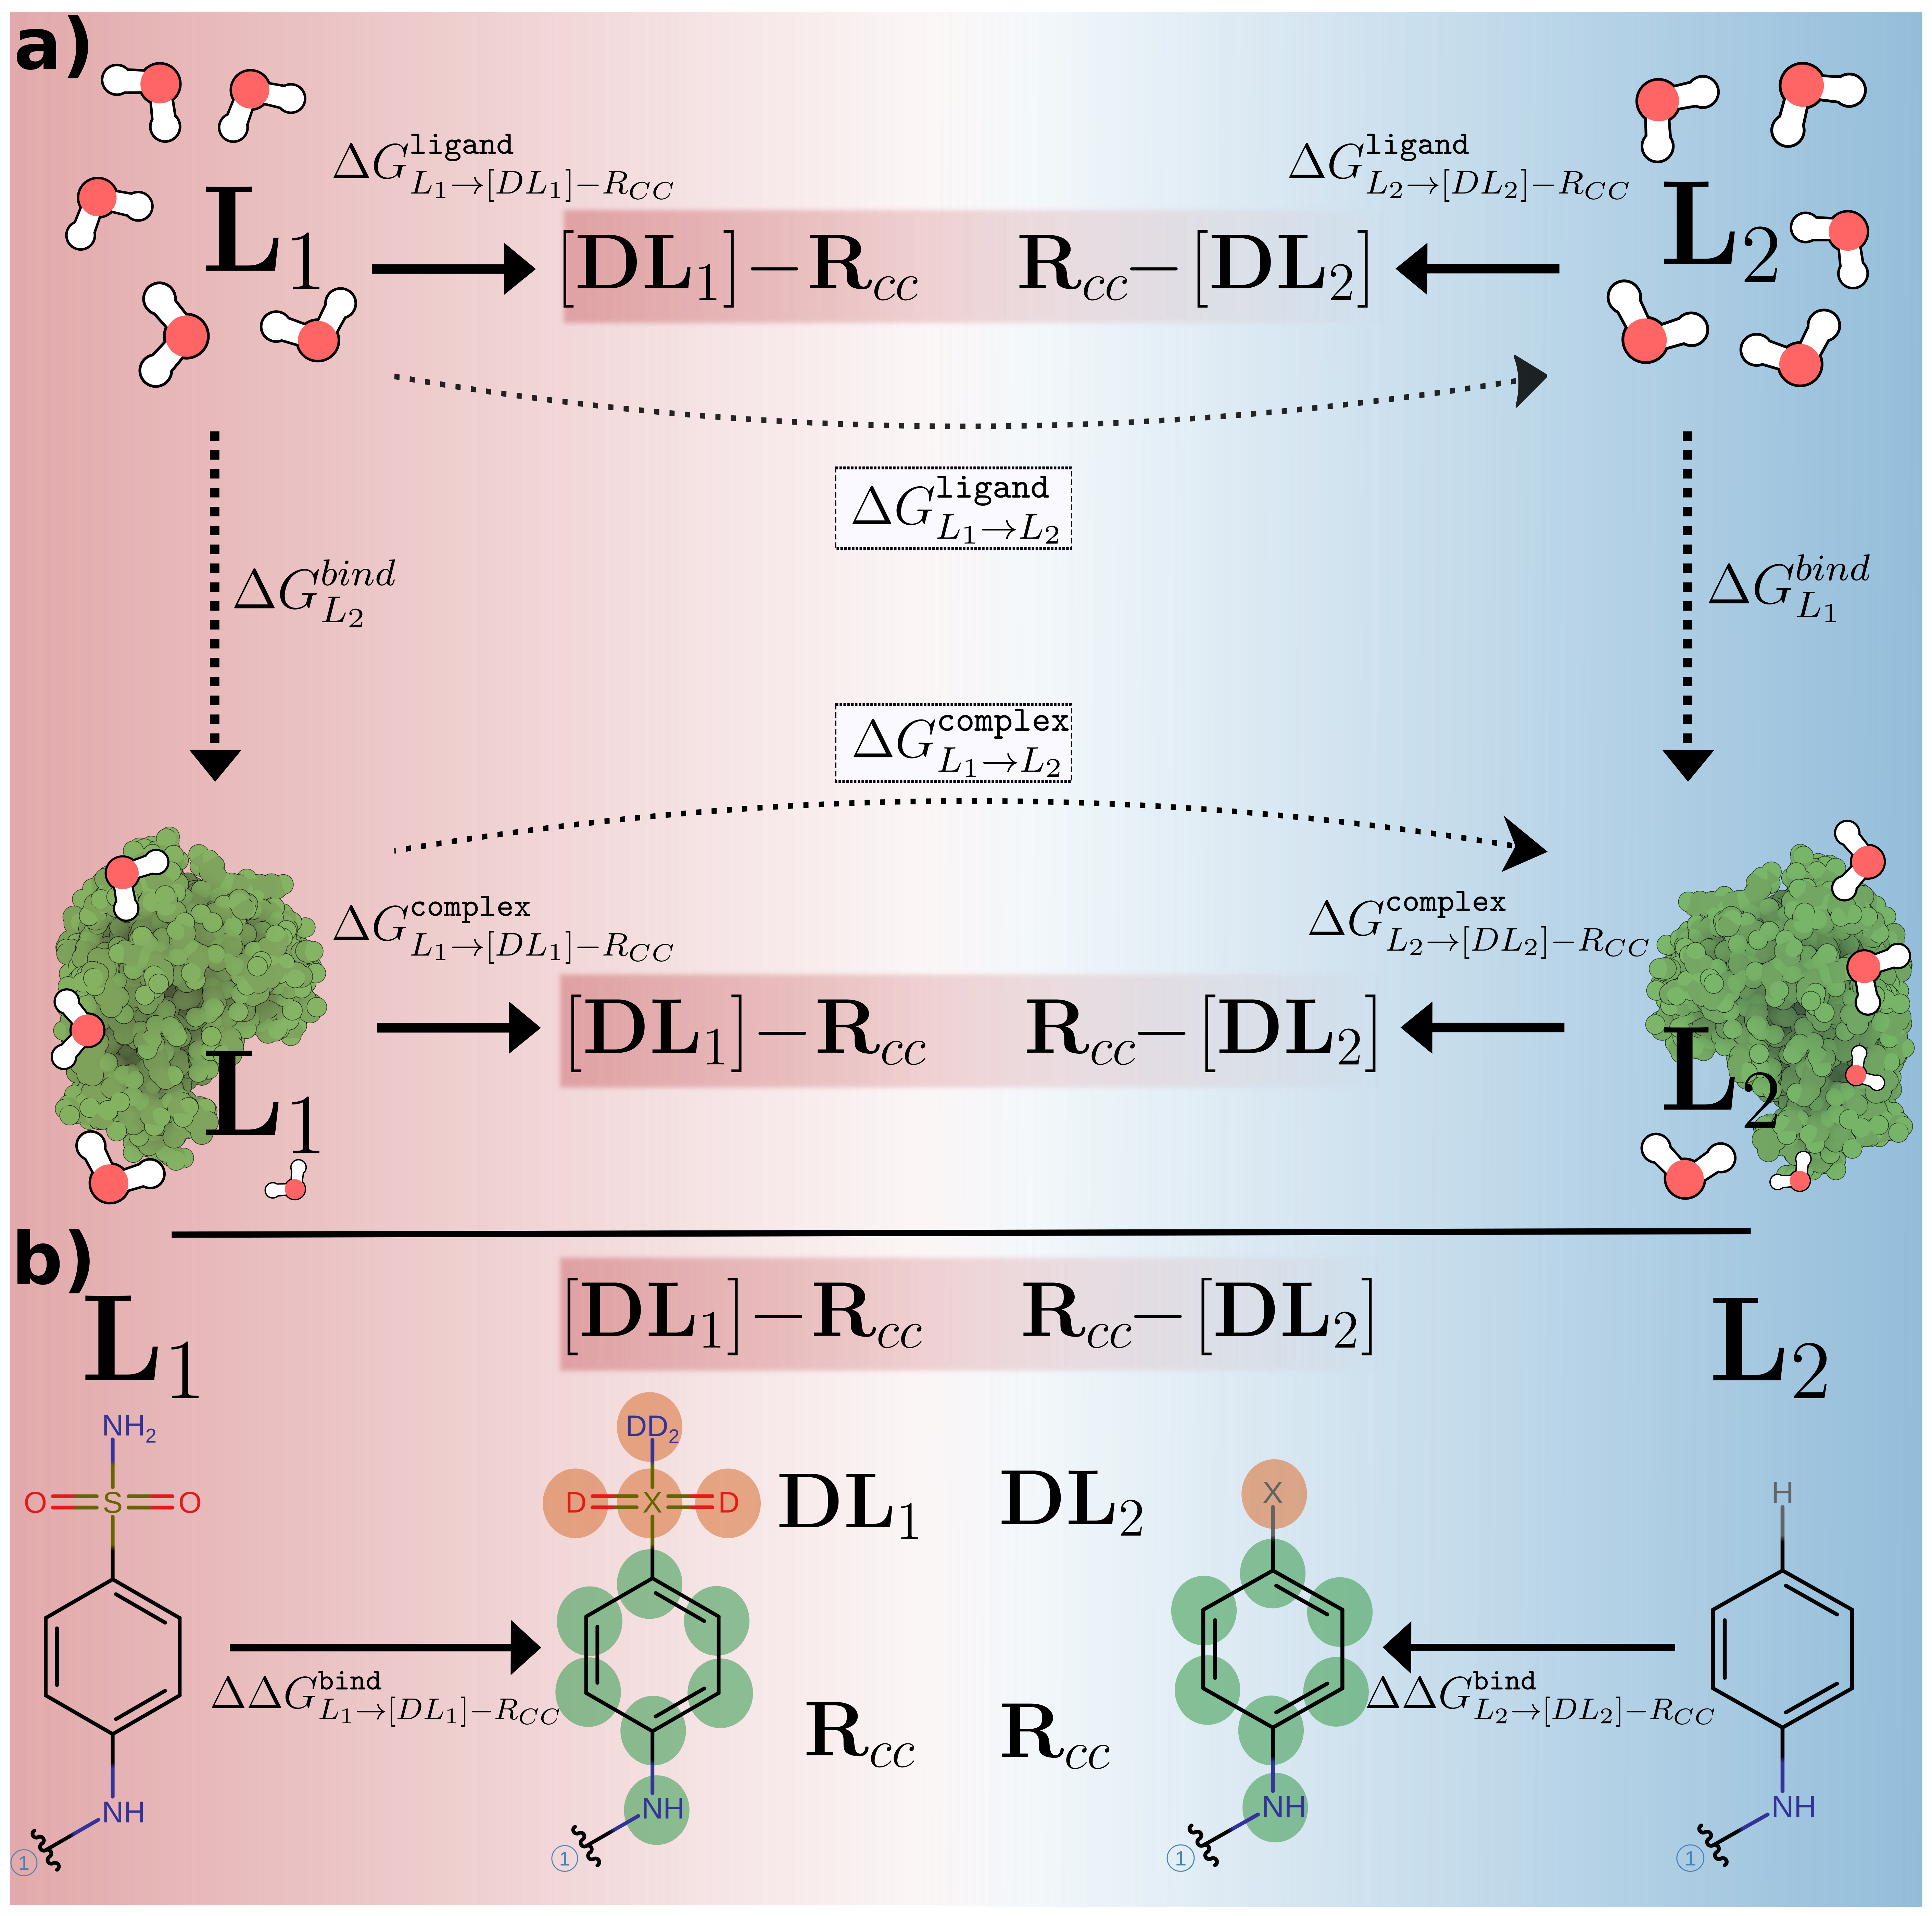
\includegraphics[width=0.7\textwidth]{alchemical_path_v5.png}
    \end{center}
    \caption{Overview of \texttt{Transformato}'s workflow}
    a) Comparison between alchemical transformations undertaken by traditional FES (dotted arrows) and the approach taken by \texttt{Transformato} (bold arrows). b) Example mutation path taken to transform two simple molecules into their common core. Green represents the common core, red those atoms that undergo mutation effects or are transferred into dummy atoms.
    \label{fig:fesvstrafo}
\end{figure}

Recently, the package \texttt{Transformato} was introduced by Karwounopoulos, Wieder, Braunsfeld, and Boresch\cite{Karwou2022Jun,braunsfeldImplementationTestingCHARMM,Wieder2022Jun}, implementing a novel approach to bypass these problems. Being a python package, \texttt{Transformato} is easy to install, use, and modify to adapt to system-specific challenges or support different MD engines. Instead of full alchemical transformations of one compound into the other, it instead relies on computing a \emph{common core} (CC) between the two physical endpoints. Summing up the energy differences between the CC and the endstates allows calculation of the free energy difference between the endstates themselves (see Fig. \ref{fig:fesvstrafo}).



With this method, atoms outside the common core are transformed into so-called \emph{dummy atoms}, a term for particles that, while still present in the simulated system, no longer have nonbonded interactions and are only kept in place by weak bonded interactions. If handled properly, these do not contribute to the calculated free energies\cite{fleckDummyAtomsAlchemical2021}.

These dummy atoms are introduced along several intermediate states, alongside various levels of scaling of nonbonded interactions. These intermediate states are then analyzed using the \emph{multistate Bennett Acceptance Ratio}\cite{shirts_statistically_2008} (mBAR), an expanded version of Bennet's acceptance ratio\cite{Bennett1976Oct}, ideally giving a close approximation of the sought relative free energy $\Delta\Delta G$. However, mBAR requires topological overlap between the various intermediate states - a problematic proposition if the ligand is liable to abscond its binding site during the simulation timeframe. To prevent this, an additional module for \texttt{Transformato} called \code{restraints.py} was developed and integrated into \texttt{Transformato}. It allows the user to either request automatic restraints or define their own. These restraints as implemented act upon the center of mass of the selected ligand atoms, restraining them to their original positions relative to the protein, with variable force.

To suit a variety of sampling needs, both harmonic and flat-bottomed energy potentials may be used as energy functions for these restraints. This way, a ligand may be specifically allowed to sample the entire binding site without being constrained, yet never leave it. This allows for better sampling and longer runtimes even at increased temperatures, without fear of losing the ligand.

An attempt at stringent validation of the methods described here was not undertaken; however, a number of qualitative simulations with a variety of testing parameters were conducted and evaluated, finding no significant impact of reasonable restraints on the calculated free energy differences.
\chapter{Theory}

\section{Theoretical Background}
Simulating the dynamics of (bio-)chemical processes (referred to as \emph{Molecular Dynamics} (MD)) in their entirety can be divided into two classes: calculations utilizing \emph{Quantum Mechanics} (QM), where interactions are calculated according to Schrödinger's Equation, and \emph{Molecular Mechanics} (MM), where calculations instead use a simplified mass-charge-force model to calculate potential energies. Combination methods (QM/MM) also exist, calculating the forces applied to the MM model using QM methods.  While there is no doubt that methods utilizing QM can deliver more accurate results (especially if using "pure" QM and not using semi-empirical methods), computational costs prohibit their use in large biological systems ("large" in this context referring to even just a single protein and its ligand) \cite{cournia_relative_2017}. Thus, for free energy calculations of the sort \texttt{transformato} is designed to accomplish, QM methods are unsuitable - which leaves MM.

This is not to say that QM has no place in MD simulations. QM is routinely used to improve geometries and improve calculation precision, with QM/MM methods allowing for enhanced accuracy while limiting computational costs, especially useful in complicated chemical environments without suitable force - fields. MD simulations based on MM also suffer from the fact that they cannot simulate the movement of electrons - meaning no bonds can break or form. This issue can be sidestepped by calculating the area of interest via QM \cite{tzeliou_review_2022}. But perhaps most importantly, the force fields used for MD simulations start out as QM calculations that are then fitted to experimental data \cite{vanommeslaeghe_charmm_2010}. Still, for this thesis, only MD based on Molecular Mechanics was used.



\subsection{Basics of Molecular Dynamics Modeling}

Since the discovery of cells, the inner workings of biological systems have always been a mystery science has raced to solve. While, of course, physical methods have allowed some degree of monitoring biochemical processes, these have significant limits - most glaringly being limited to physically-present structures. With Molecular Dynamics (MD) on the other hand, it is entirely possible to observe molecular interactions as they would happen in reality - at the leisure and convenience of the observer, with an unmatched resolution and clarity, and without the need to synthesize a single atom - the so-called \emph{in silico} - approach.

In general, MD aims to simulate the movement of atoms in a molecular system over time, governed by the physical interactions present in the molecule \cite{Hollingsworth2018Sep}. Unlike QM, which tries to calculate interactions using various approximations or even solutions of the Schrödinger equation, MM simulations are inherently uncertain. Forces are approximated by what are essentially the mechanical principles of Newton: Atoms are perfect spheres, with mass and charges, and all their interactions are defined by a set of forces governing the interactions of specific types of atoms. As such, the kinetic energy $K$ of an MD system is simply the kinetic energy of its atom masses $m_i$  at speed $v$, using the equation familiar from Netwonian mechanics (Eq. \ref{eq:kinenergy}), while their potential energy is defined by the potentials governing their interactions.
\begin{equation}\label{eq:kinenergy}
    K=\sum_i\frac{m_i v_i^2}{2}
\end{equation}

\paragraph{Force Fields}
For almost all force fields, forces in MM simulations may be divided into two categories - \emph{bonded} and \emph{nonbonded} interactions. These are often used synonymously with \emph{intramolecular} and \emph{intermolecular} forces, but are far from the same - it is quite possible, and especially in biological systems the rule more than the exception, that nonbonded but intramolecular interactions contribute a significant part to the protein structure, with electrostatic forces and the hydrophobic effect being especially important for protein folding and thus functionality \cite{kumar_close-range_2002}.

Bonded forces are generally given explicitly for each atom type. They are:
\begin{itemize}
    \item Bonds (across two atoms)
    \item Angles (the angle across three atoms)
    \item Dihedrals (the angle across four atoms)
    \item Impropers (also called \emph{improper dihedrals}, the angle of a fourth atom being out-of-plane with the other three)
    \item Urey-Bradley (sometimes grouped with the angle terms; describes noncovalent bonds over larger distances)
\end{itemize}

All these are stored in \emph{parameter files}, which contain the force parameters for each of these.

\begin{figure}
\small
\begin{verbatim}
BONDS
CG1N1  CG2R51  375.00     1.4220 ! DCG, yxu, RNA
CG1N1  CG2R61  345.00     1.4350 ! 3CYP, 3-pyridine (PYRIDINE pyr-CN)

ANGLES
CG2R51 CG1N1  NG1T1    40.00    180.00 ! DCG, yxu, RNA
CG2R61 CG1N1  NG1T1    40.00    180.00 ! 3CYP, 3-pyridine (PYRIDINE pyr-CN)

DIHEDRALS
NG1T1  CG1N1  CG2R61 CG2R61  0.0100 2    0.00 ! CNP2, by ac_aa
NG1T1  CG1N1  SG311  CG321   0.0060 1    0.00 ! XCN, by ac_aa

IMPROPERS
CG2D1  CG331  NG2D1  HGA4      25.00  0     0.00 ! SCH1, xxwy
CG2D1  CG331  NG2P1  HGR52     18.00  0     0.00 ! SCH2, xxwy

\end{verbatim}
   \caption{Illustrative excerpt from a parameter file created by CGenFF with a few definitions for bonds, angles dihedrals and impropers each.}
    \label{fig:parmfile}
\end{figure}

As apparent in figure \ref{fig:parmfile}, force-field parameter files are structured very simply: The first few columns define the "atom types" for which a given set of parameters is valid. The others define the numeric value of the various parameters for the potential; for simple bonds for example the first value denotes the force constant, and the second the equilibrium distance. These values are inserted into a harmonic potential and then used to calculate the force. 


In a MD system, the combined potential energy is simply the sum of bonded and nonbonded potential energy terms, both of which are dependent on the relative positions $(\Vec{r})$ of the atoms. Transformato uses the Charmm General Force Field\cite{vanommeslaeghe_charmm_2010}.

The sum for bonded potentials is the sum of the individual potentials, whereas the nonbonded potentials \emph{generally} consist of electrostatic (Morse) and VdW (Lennard-Jones) potentials.


However, these equations do not offer the information we require. What we want is the movement of atoms across the time dimension (thus Molecular \emph{Dynamics}). However, these potentials are a significant part of the way there. To simulate a MM system, all atoms are assigned  random initial velocities. For each step, the forces resulting from bonded and nonbonded interactions are calculated and applied to these atoms in a  manner resembling classical mechanics. The atoms are then moved as dictated by their momentum and the timestep chosen, and the cycle repeated. QM/MM differs from classical MM in the way the forces are calculated: while the interactions are still governed by classical mechanics, the force contributions are derived form quantum mechanical calculations rather than the simple force potentials used in MD.


Following these steps results in positions for each atoms for every step you calculate. By combining these into a single file you get a \emph{trajectory}, containing the movements of your atoms along the entire simulation. However, trajectories typically do not contain every single calculated position, but rather only every n-th step, as trajectory files would otherwise be prohibitively large.

\subsection{Relative and absolute binding free energies}

Calculating the free energies from these trajectories, however, requires additional steps. For our purposes, we need to differentiate two types of free energy differences:
\begin{itemize}
    \item \emph{absolute} free energies ($\Delta G_{bind}$); Here, the ligand energy difference is between the ligand bound in complex, and the ligand free to explore all other possible configurations.
    \item \emph{relative} free energies ($\Delta\Delta G^{A\rightarrow B}_{bind}$): Here, the ligand energy difference is compared between two specific states $A$ and $B$.
\end{itemize}

\begin{figure}[H]
   
    
    

  \begin{center}

    \tikz{%
      \node[outer sep=1mm](L1A) at (0,0) {$\mathrm{(P\cdot{}L1})_{aq}$};
      \node[outer sep=1mm](L2A) at (6,0) {$\mathrm{(P\cdot{}L2})_{aq}$};
          \node[outer sep=1mm](L1G) at (0,3) {$\mathrm{{\color{gray}P}+(L1})_{aq}$};
              \node[outer sep=1mm](L2G) at (6,3) {$\mathrm{{\color{gray}P}+(L2})_{aq}$};
                  \draw[-{Stealth},uniwine,ultra thick](L1A) -- node[below,outer sep=3mm]{$\Delta A^{\mathit{L1\rightarrow L2}}_{\mathit{bound}}$} (L2A);
                  \draw[-{Stealth},uniwine,ultra thick](L1G) -- node[above,outer sep=3mm]{$\Delta A^{\mathit{L1\rightarrow L2}}_{\mathit{free}}$} (L2G);
                  \draw[-{Stealth},uniblue,ultra thick](L1G) -- node[right]{$\Delta A^{\mathit{L1}}_{\mathit{bind}}$} (L1A);
                  \draw[-{Stealth},uniblue,ultra thick](L2G) -- node[right]{$\Delta A^{\mathit{L2}}_{\mathit{bind}}$} (L2A);
                  }
    
    \caption[Thermodynamic cycle for RBFE differences]{A classic thermodynamic cycle to calculate free binding energy differences $\Delta A_{binding}$ between ligands $L_1$ and $L_2$. The physical path is marked in blue; the alchemical one in wine red.} 
    \label{fig:thermocycle_rbfe}
  \end{center}
\end{figure}

Calculating them typically exploits thermodynamic cycles. In Fig. \ref{fig:thermocycle_rbfe} you can see a typical example of such a cycle to calculate relative \emph{binding} free energies: two different Ligands $L_1$ and $L_2$ are in aqueous solution with the same Protein $P$. The quantity of interest is the relative binding free energy $\Delta \Delta A_{bind}$, which can easily be calculated by using the nonphysical - \emph{alchemical} transformations marked in red (Eq. \ref{eq:deltadeltaAbind}). While it would, theoretically, be possible to calculate $\Delta A^{L1}_{bind}$ directly, doing so still requires massive amounts of computational power and research time, making it prohibitive for typical usage \cite{fujitani_direct_2005}.

\begin{equation}
    \Delta \Delta A_{bind} = A^{L2}_{bind}-A^{L1}_{bind}=A^{L1\rightarrow L2}_{bound}-A^{L1\rightarrow L2}_{free}
    \label{eq:deltadeltaAbind}
\end{equation}


For the alchemical transformations however, all that needs to be done is to replace one ligand binding to the protein with the other. Doing so directly, however, does not work (well). Calculating free energies requires \emph{phase space overlap}. \emph{Phase space} in this context refers to the total allowed set of positions and momenta of the system. Two completely different ligands will overlap barely, if at all - giving error bars bigger than the calculated energy difference. Thus, the amount of changes in the calculation needs to be reduced by introducing \emph{intermediate states}. Free Energy differences are then not calculated between the endstates, but rather as sum of energy differences between the endstates (Eq. \ref{eq:sumintstates}). This allows for much more overlap between the individual states, leading to much smaller margins of error in total.

\begin{equation}
    \Delta A_{1,K} = \sum^{K-1}_{i=1} \Delta A_{i,i+1}
    \label{eq:sumintstates}
\end{equation}



\begin{figure}[h]
    \centering
     

    \tikz{%
      \node[outer sep=1mm](S1A) at (0,0) {$\mathrm{(S1)}_{aq}$};
      \node[outer sep=1mm](S2A) at (6,0) {$\mathrm{(S2)}_{aq}$};
          \node[outer sep=1mm](S1G) at (0,3) {$\mathrm{S1}$};
              \node[outer sep=1mm](S2G) at (6,3) {$\mathrm{S2}$};
                  {\draw[-{Stealth},uniwine,ultra thick](S1A) -- node[below,outer sep=3mm]{$\Delta A^{\mathit{S1\rightarrow S2}}_{\mathit{aq.}}$} (S2A);}
                  {\draw[-{Stealth},uniwine,ultra thick](S1G) -- node[above,outer sep=3mm]{$\Delta A^{\mathit{S1\rightarrow S2}}_{\mathit{gasp}}$} (S2G);}
                  \draw[-{Stealth},uniblue,ultra thick](S1G) -- node[right]{$\Delta A^{\mathit{S1}}_{\mathit{solv}}$} (S1A);
                  \draw[-{Stealth},uniblue,ultra thick](S2G) -- node[right]{$\Delta A^{\mathit{S2}}_{\mathit{solv}}$} (S2A);
                  }


    \caption[Thermodynamic cycle for RSFE differences]{A classic thermodynamic cycle to calculate free solvation energy differences $\Delta\Delta A_{solvation}$ between two substances $S_1$ and $S_2$ in gaseous phase and aqueous solution, with physical paths in blue and alchemical paths in wine red.}
    \label{fig:thermocycle_rsfe}
\end{figure}


The same approach also enables calculating relative \emph{solvation} free energies. Here, the "physical" path leads from an unsolvated compound to a solvated one, whereas the alchemical pathways again lead through simply changing the compound (Fig. \ref{fig:thermocycle_rsfe}).

\subsection{Generation of intermediate states and dummy atoms} \label{sec:intstatesanddummys}

The simplest method of generating intermediate states as used in Eq. \ref{eq:sumintstates} is to linearly "mix" the  potentials of the endstates 0 and 1 $U_\lambda$ from $U_0 \rightarrow U_1$, with $\lambda$ being known as the \emph{coupling parameter}. Notably, $\lambda$ only affects a subset of potentials (usually nonbonded interactions, meaning charges and Lennard-Jones-interactions, will be most heavily affected), while most of the potential remains unaffected. The total potential for a given intermediate state $i$ as required by Eq. \ref{eq:sumintstates} is thus as given by Eq. \ref{eq:totalpotential}, usually with $U_0; U_1 << U_{environment}$.
\begin{equation}
U^{total}_i   = (1-\lambda)U_0 + \lambda U_1  + U_{environment}
\label{eq:totalpotential}
\end{equation}
This kind of linear scaling, however, creates a number of problems; most pressingly a distinct lack of phase space overlap required for analysis resulting from the van-der-Waals endpoint problem (see section \ref{sec:vdwproblem}). \texttt{Transformato} does \emph{not} use these kinds of "$\lambda$-scaling" methods, instead opting for an approach called "serial atom insertion" (see section \ref{sec:tf_principles}).

An even more egregious problem arises when the number of atoms changes between endstates: Typical implementations of statistical thermodynamics as required for MD do not allow for changing the number of particles in the system. To sidestep this problem, \emph{dummy atoms} are introduced by turning off all interactions but their bonded terms - either just for surplus atoms (known as the \emph{single topology approach}) or by having both topologies fully present in all states, with the currently unused one handled as dummy atoms (known as the \emph{dual topology approach}). It has been shown that, used correctly and provided they remain well-defined in position and orientation, their influence on calculated energies is zero as their terms in $\Delta \Delta A$  cancel each other out\cite{fleckDummyAtomsAlchemical2021}. This allows the system to retain a constant number of particles.

\subsection{Intermediate state analysis, postprocessing and calculation of free energy}

But one question has so far remained unanswered: how to actually get to $\Delta A_{i,i+1}$ from Eq. \ref{eq:sumintstates}? 
FES conducted by the methods above typically rely on either Thermodynamic Integration (TI) \cite{straatsma_free_1986} or Bennett's Acceptance Ratio (BAR) \cite{Bennett1976Oct,shirts_statistically_2008} to analyse the results from the various intermediate states, both of which start from the identity of free energy (Eq. \ref{eq:identityoffreenergy}), which defines the energy difference between two states $i,j$ as dependent on the logarithm of the \emph{partition functions} $Q_{i,j}$.
\begin{equation} \label{eq:identityoffreenergy}
    \Delta A_{i,j}=-k_{B}T\cdot \ln\frac{Q_i}{Q_j}
\end{equation}
These partition functions describe the thermodynamic properties of the system dependent on the used \emph{ensemble}, the set of possible states the system can have while exchanging energy with the outside world in a state of thermal equilibrium. For this thesis, all simulations were conducted using an \textbf{NPT} ensemble, meaning the \textbf{number} of particles, and the average \textbf{pressure} and \textbf{temperature} of the system were held constant. Eq. \ref{eq:nptpartition} is the partition function for the  \emph{canonical} or NVT ensemble (the derivation for the NPT ensemble follows the same pattern, but gives Gibbs instead of Helmholtz free energies). As can be seen, the function integrates over the entire phase space volume $\Gamma$, allowing derivatives to express a single expected value (represented by $\langle \rangle$).
\begin{equation} \label{eq:nptpartition}
    Q=\int_\Gamma e^{-\frac{U(\Vec{q})}{k_B T}d\Vec{q}}
\end{equation}

\paragraph{Thermodynamic Integration} Of the two methods, TI is  the older one. It relies on simply integrating the total potential energy $dU$ over the coupling factor $d\lambda$ as shown in Eq. \ref{eq:ti_integration}. However, as we cannot calculate the integral in a continous manner for $\lambda =[0\rightarrow1]$, a numeric approximation as shown in Eq. \ref{eq:ti_approximation} is required, where the difference of free energy is given as the sum of the integral for actually calculated states $K$, each weighted according to the weight factor $w_k$. $w_k$ may be computed a number of different ways; the common all-purpose method is the trapezoidal method. The weighting method should be choosen carefully, as it has significant impact on result quality \cite{boresch_efficiency_2011}.

\begin{equation} \label{eq:ti_integration}
    \Delta A=\int_0^1 \biggl \langle\frac{dU(\lambda,\Vec{q})}{d\lambda} \biggr \rangle_{\lambda} d\lambda 
\end{equation}
\begin{equation} \label{eq:ti_approximation}
    \Delta A \approx \sum_{k=1}^K w_k \biggl \langle\frac{dU(\lambda,\Vec{q})}{d\lambda} \biggr \rangle_{k}
\end{equation}
While the calculation is rather simple, there are a few significant drawbacks to TI. First, it requires the computation of $\frac{dU}{d\lambda}$ for all $\Vec{p}$, which requires a MD engine with facilities capable of the appropriate derivations. Secondly, TI does badly with sudden steps in the integral, requiring either a highly efficient numeric integrator, the use of techniques increasing phase space overlap (such as soft-core potentials) or resulting in large uncertainties. It should be noted that this, alongside a lack of continuous, defined $\lambda$ makes it unsuitable for the Serial-Atom-Insertion approach used in \texttt{Transformato} (see section \ref{sec:tf_principles}).


\paragraph{Bennett's Acceptance Ratio} BAR and its multistate extension mBAR on the other hand do not face such limitations, at the cost of significantly increased complexity. First a set of weighting functions $\alpha_{i,j} (\Vec{q})$ are generated for the overlap space of the state variables $K \times K$. The actual derivation then starts from the same identity of free energy (Eq. \ref{eq:identityoffreenergy}) as TI, but by introducing the weighting factor, an equivalency between $Q_i$ and $Q_j$ can be expressed (Eq. \ref{eq:mbareq}).
\begin{equation} \label{eq:mbareq}
    Q_i\langle \alpha_{i,j} e^{-\beta U_j}\rangle_i = Q_j \langle \alpha_{i,j} e^{-\beta U_i} \rangle_j
\end{equation}
Introducing the empirical estimator $\langle g \rangle_i = N_i^{-1} \sum_{n=1}^{N_i} g(\Vec{q_i},n)$ allows to write the equivalency in Eq. \ref{eq:mbareq} as a sum (Eq. \ref{eq:bar_sum}). Through the use of a \emph{numerical bridge integrator} \cite{tan_likelihood_2004} it is possible to arrive at the free energy equation \ref{eq:bar_freeenergy}. Notably, this equation actually gives a \emph{single} free energy instead of an energy difference; however the use of an undefined additive constant means that all calculations need to be put in reference to the energy of one of the states (typically the starting endpoint), again arriving at an energy difference.
\begin{equation} \label{eq:bar_sum}
    \sum^K_{j=1}\frac{\hat{Q}_i}{N_i} \sum_{n=1}^{N_i} \alpha_{i,j} e^{(-\beta U_j(\Vec{q_i},n))} = \sum^K_{j=1}\frac{\hat{Q}_j}{N_j} \sum_{n=1}^{N_j} \alpha_{i,j} e^{(-\beta U_i(\Vec{q_j},n))}
\end{equation}
\begin{equation} \label{eq:bar_freeenergy}
\hat{A_i}= -\beta^{-1} \ln{\sum^K_{j=1} \sum^{N_j}_{n=1}\frac{e^{(-\beta U_i)}}{\sum^K_{k=1} N_k e^{\beta \hat{A_k}-\beta U_k}}}   
\end{equation}
Unlike TI, BAR and mBAR are able to give accurate results even with significant changes to $K$ and correspondingly little phase space overlap. Notably, it is able to deal with the significant changes caused by the Serial-Atom-Insertion method used by \texttt{Transformato} and is thus used to calculate the free energies of interest.
\subsection{Soft-core potentials and the van-der-Waals endpoint problem} \label{sec:vdwproblem}
In a standard MD simulation, the Lennard - Jones potential $U_{LJ}$ is given by formula \ref{eq:ljstandard}, with $r$ as interparticle distance, and $A;B$ as atom-type dependent constant factors.
\begin{equation}
U_{LJ}(r,\lambda)=(1-\lambda)(\frac{A}{r^{12}} - \frac{B}{r^6}) \label{eq:ljstandard} \\
\end{equation}
This usually works rather well -  the shape of the potential ensures that no two LJ particles inhabit the same spot. However, free energy calculations, for the reasons discussed in section \ref{sec:intstatesanddummys}, usually require the presence of \textit{dummy atoms} - which obviously do not have Lennard - Jones interactions. It's here where problems may now occur -  as there are no LJ interactions, atoms may move freely into each other. This may not seem like such a significant problem - but forces still need to be calculated. Should particles manage to inhabit the exact same position, this would result in a division by zero - problematic, but most modern MD software can handle this. 


Both more problematic and more common, however, is the case that two particles get very close to each other. This is especially common in simulations with linear coupling between $\lambda$ and the LJ potential, as for low values of $\lambda$ the interaction range may decrease to such an extent that a particle may skip the entire "well" of the potential, and directly encounter its "wall", leading to extremely high forces being applied \cite{boresch_avoiding_2011}. (see Fig. \ref{fig:ljandsoftcore}). In this case, (i) the derivative $\langle \frac{\delta U}{\delta\lambda} \rangle$ may diverge, and (ii) because of the sudden change in energy the entire simulation may become unstable. This is known as the \textit{van-der-Waals endpoint problem} (or \textit{-catastrophe}, for the more dramatically inclined).

\begin{figure}
    \centering
    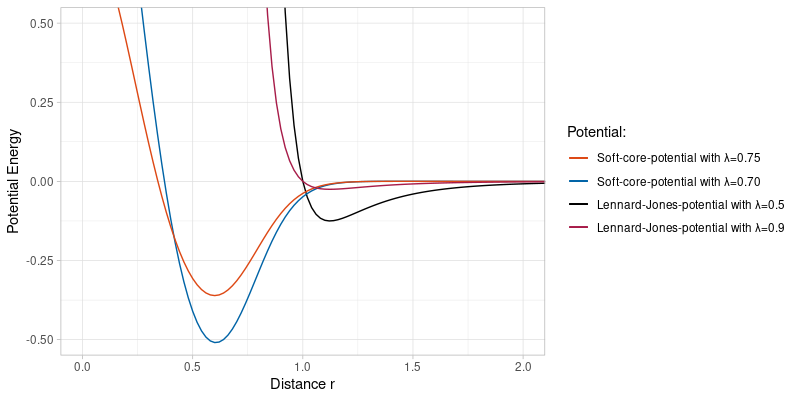
\includegraphics[height=6cm]{LJandsoftcore.png}
    \caption[Comparision between behaviour of standard LJ potentials vs. soft-core potentials]{Comparison between behaviour of standard Lennard-Jones and soft-core potentials for various states of $\lambda$. Visibly: For the standard LJ potential, well size decreases with increasing $\lambda$, while steepness of the potential wall increases. The reverse is true for soft-core potentials, which also remain defined at $r=0$}
    \label{fig:ljandsoftcore}
\end{figure}

To avoid this problem, soft-core potentials dependent on the coupling factor $\lambda$ were introduced as shown in Equation \ref{eq:ljsoftcore}\cite{Beutler1994Jun}:
\begin{equation}
U_{LJ}^{SC}(r,\lambda)=(1-\lambda)(\frac{A}{(r^2 +\lambda \delta)^6 }-\frac{B}{(r^6 +\lambda \delta)^3})
\label{eq:ljsoftcore}
\end{equation}
These mostly solve the problem, as there can now be no division by zero and the fractions remain finite in all circumstances. They can, however, be computationally expensive  - especially for MD engines lacking native support for them\cite{Li2020Aug}. It is important to note that \texttt{Transformato} for this reason does \textbf{not} use soft-core potentials, but rather the "serial-atom-insertion" approach (see section \ref{sec:tf_principles}).


\section{The common-core serial-atom-insertion framework {\texttt{Transformato}}}
To avoid these problems and reduce general computational cost of FES, the common-core serial-atom-insertion framework \texttt{Transformato} was conceptualized and implemented. Being engine-agnostic - its outputs theoretically being computable with any of the widely-used Molecular Dynamics engines (openMM, CHARMM, AMBER, GROMACS, etc.). Currently, while the outputs are computable with any MD engine, \texttt{Transformato}  only provides output scripts for openMM and CHARMM. Within these limitations however, it allows straightforward calculation of relative binding and solvation free energy differences in the form of a single, easy-to install python package.


\subsection{Theoretical Principles} \label{sec:tf_principles}
\texttt{Transformato} is built on two distinct theoretical pillars: The \emph{Serial Atom Insertion} approach to generating intermediate states, and the \emph{Common-Core} approach to handling thermodynamic cycles, together referred to as the "serial-atom-insertion common-core" method (SAI/CC).

\emph{Serial Atom Insertion} (SAI)\cite{boresch_avoiding_2011} refers to an alternative method of avoiding the van-der-Waals-Endpoint problem without relying on the soft-core potentials discussed in section \ref{sec:vdwproblem}, developed by Boresch and Bruckner in 2011. This allows for a significant decrease of computational cost in MD engines without native, GPU-assisted soft-core modelling, at the drawback of having significant, stepwise changes to the states present in phase space, making it unsuitable for analysis via Thermodynamic Integration. Central to this method is to turn off the changed atoms in successive fashion, rather than scaling all of their interactions as one $\lambda$-dependent potential to generate the intermediate states. Thus, rather than depending on potentially very small $\lambda$ values (Eq. \ref{eq:nonsai} for the simplest case, outlined in section \ref{sec:intstatesanddummys}), the total potential energy is calculated by having the each atom turned on or off be its own intermediate state, with no intermediate scaling of the nonbonded parameters (Eq. \ref{eq:saipot}, for a molecule in solution with $M$ Lennard-Jones particles, itself containing $m$ particles with $u^{LJ}_{i,j}$ denoting the Lennard-Jones interaction between two particles).

\begin{equation}\label{eq:nonsai}
    U(\lambda)=\sum_{1\leq i<j \leq M} u^{LJ}_{i,j}+\lambda \sum_{1 \leq i \leq M} \sum_{1 \leq l \leq m} u^{LJ}_{i,j} \hspace{2cm} \lambda=[0,1]
\end{equation}
\begin{equation}\label{eq:saipot}
    U(k)=\sum_{1\leq i<j \leq M} u^{LJ}_{i,j}+\sum_{1 \leq i \leq M} \sum_{1 \leq l \leq k} u^{LJ}_{i,l} \hspace{2.3cm} k=[0,m]
\end{equation}

The term \emph{Common Core} \cite{Wieder2022Jun,braunsfeldImplementationTestingCHARMM} refers to the atypical alchemical path taken by \texttt{Transformato}. Whereas traditional FES transform the endstates directly into each other, \texttt{Transformato} instead transforms each of them into their maximum common topology - the \emph{Common Core}. 

Routing via the common core is useful, as the complete free energy difference between two ligands on the alchemical pathway (illustrated in Fig. \ref{fig:thermocycle_rbfe}) can be expressed as the sum of the individual free energy differences (Eq. \ref{eq:sumofligandtocc}).
\begin{equation}\label{eq:sumofligandtocc}
    A^{L_1\rightarrow L_2}_{bound}=\Delta \Delta G_{bound}^{L_1\rightarrow L_2}=\Delta \Delta G^{L_1\rightarrow [D_{L_1}]-R_{CC}}_{bound}-\Delta \Delta G^{L_2\rightarrow [D_{L_2}]-R_{CC}}_{bound}
\end{equation}
To reach the common core, the \emph{mutation path} is generated by the program from each ligand $L_1, L_2$ to the CC $R_{CC}$, along which atoms not belonging to the CC are decoupled and transformed into dummy atoms. First, electrostatic interactions are turned off, followed by Lennard-Jones interactions of first hydrogen, then separately non-hydrogen atoms successively. The last atom connecting the \emph{dummy regions} $DL_1,DL_2$ with the CC is called the \emph{terminal junction} X. Interaction terms involving X are scaled linearly to have the bond specifications of $L_1$ match those of $L_2$. As the SAI/CC requires redistribution of charges\footnote{The sum partial charge of the terminal junction at the end needs to be 0 to cancel itself out across the thermodynamic cycle, see \cite{Karwou2022Jun,Wieder2022Jun} for details}, this atom retains some Lennard-Jones interaction and forms the anchor point for the dummy region. Each stage of this mutation forms an intermediate state similar to those used with $\lambda$-scaling methods, though not dependent on a numeric factor. After each intermediate state is simulated, $U_{i,j}$ may be calculated in postprocessing, allowing the calculation of free energy differences via mBAR. This is done both for the ligand in complex with the protein, as well as for the ligand in simple solution, allowing calculation of $A^{L_1\rightarrow L_2}_{bound}$ via exploitation of the cycle in Fig. \ref{fig:thermocycle_rbfe}.

It should be noted the two methods are independent from each other; it is quite possible to compute a direct transformation using SAI or to use the CC approach alongside soft-core potentials, with increasing adoption of native soft-core methods in MD engines making the latter especially a useful proposition. However, this is as of yet not implemented in \texttt{Transformato}.
\subsection{Theoretical considerations for Restraints in \texttt{Transformato}}
While \texttt{Transformato} yields excellent results for almost all test systems, problems may arise in unstable systems with a ligand prone to leaving the binding site of its associated protein within the timeframe of the simulation. This may even be a problem in comparatively stable systems, assuming a larger-than-usual timeframe is desired. To circumvent this, restraints need to be applied within the system, keeping the ligand within the binding site while still allowing sampling within it. However, irrespective of other considerations, the addition of restraints must not influence the calculated free energy differences, as this would render the entire exercise pointless. Restraints as implemented act as bonded force, and are a simple addition to the sum forming $U_{bonded}$. Given that the free energy is directly dependent on $U$ via the partition functions (Eq. \ref{eq:nptpartition}) and the pathway energy results from the subtraction of the $L_2$ pathway from the $L_1$ pathway (Eq. \ref{eq:sumofligandtocc}), this means that $U^{restraints}_{L_1}$ must be equal to $U^{restraints}_{L_2}$ for the restraints to cancel each other out.

However, this is not possible for restraints involving the entire system. In case of a simple harmonic restraint as given by Eq. \ref{eq:simpleharmonic}), with $r$ the distance between the restrained particles - one anchored on the ligand, one anchored to the protein -, $r_0$ the equilibrium distance, and $k$ the force constant,  the amount of energy added to the system is proportional to the movement of the restrained systems vis-a-vis each other.
\begin{equation}\label{eq:simpleharmonic}
    U^{rest}=0.5\cdot k(r-r_0)^2 
\end{equation}
To achieve $\langle U^{rest}_{L_1}\rangle == \langle U^{rest}_{L_1}\rangle$, the first condition is the same number of restraints in the system. However, as $\langle U \rangle$ is dependent on $r$, the expectation value for $r$  also must not change. As $r$ is dependent on the atom interactions and thus its given force field parameters, that means that the restraint needs to be connected to the same atom types (or groups of atom types) at both endstates. The current implementation in \texttt{Transformato} achieves this by restricting its restraints to the common core, as that represents a useful list of atoms that will both remain constant during the mutations and have the same atom type in both ligands, barring the terminal junction.

However, the common core does not exist in a vacuum, and $r$ is dependent not only on movement by the ligand, but that of the protein as well. To satisfactorily keep ligands restrained in the binding site while still allowing for low enough force constants to facilitate sampling, current automatic restraints anchor to protein carbon-alphas near the ligand. These are affected by the ligand, with different ligand structures producing different effects. These differing interactions will also have differing effects on the movement of the common core structures, further diverging $\langle (r-r_0) \rangle$ between $L_1$ and $L_2$. While the anchoring of the restraints exclusively to alpha carbons is an attempt to minimize this and contributions are likely to be small, is is nevertheless an inaccuracy introduced into the calculations.

To minimize this inaccuracy, restraints may simply be turned off for the endstates. With mBAR, as the $\hat{A}_i$ is formed from the sum differences between two adjacent states (Eq. \ref{eq:bar_freeenergy}), as long as the restraints are introduced away from the endstates, their energy contribution is considered in $\Delta \hat{A}_{1}\rightarrow \hat{A}_{2}$ at both sides instead of being part of the initial system. As the contribution at the common core is necessarily the same, the terms thus cancel each other out. \texttt{Transformato} provides the keyword \code{scaling} for this, which scales $U^{restr}$ linearly across the first four intermediate states, with the endstates receiving no contribution at all.

On the topic of contribution, harmonic restraints as in Eq. \ref{eq:simpleharmonic} suffer the disadvantage of always having a contribution to the total potential, as given the high numerical precision of simulations along with initial velocities assigned at the start of the system means that $r-r_0$ never evaluates to 0. Similarly, the harmonic shape of the restraint means that a restraint capable of stopping escape from a binding site will have significant contributions even within that binding site, discouraging sampling and possibly introducing errors into the energy calculations that way. To alleviate this, it is recommended to instead use one of the provided flat-bottom potentials, e.g. Eq.\ref{eq:flatbottom}.
\begin{equation}\label{eq:flatbottom}
    U^{rest}=k \cdot step(|r-r_0|-wellsize) \cdot (r-r_0)^2
\end{equation}
With $r$ once again representing distance, $r_0$ being the equilibrium distance and $k$ the force constant. New additions are the $wellsize$ and a $step$ function. The wellsize represents a radius around the equilibrium distance which the restraint is free to move around in. As long as the expression $|r-r_0|-wellsize$ evaluates negative, $step(x)=0$. Should it however evaluate positive, meaning that the restraint has left the well, the step function evaluates to 1 and the standard harmonic restraints are applied. This allows definition of fairly stringent restraints without impact on sampling within the binding site.
\subsection{Installation and Usage}\label{sec:installation}
Installing \texttt{Transformato} is fairly straightforward: it requires a working installation of \texttt{conda} and \texttt{python}. Using \texttt{git clone}, download the package from the repository\footnote{\url{https://github.com/wiederm/transformato}} and run \texttt{python setup.py install}. Install the \texttt{conda} environment called \texttt{fep} consisting of \texttt{Transformato} and all its dependencies, located in \code{transformato/test\_environments/}. Activate the environment and you're done.

To calculate free energies, retrieve a PDB containing your ligand-protein complex for one endpoint, then modify the ligand to suit your purposes, using e.g. CHARMM-GUI's\footnote{\url{https://www.charmm-gui.org/}} ligand builder. For each endpoint, solvate once the complex including the ligand and once just the ligand using e.g. CHARMM-GUI's Solvation Builder. Take the output folders, equilibrate them and name the 'complex' and 'waterbox', respectively. You will then need to create a config.yaml file containing the names of your structures and parameters you want your simulation to have - any restraints you wish to apply must also be defined here. The simplest case for specifying restraints is simply done by adding the keyword \code{restraints: auto} to the \emph{simulation} part of the configuration file. This restrains the entire ligand backbone via its center of mass to the center of mass of the protein backbone. Inside the code, this is referred to as \texttt{simple} mode. Another possibility is the generation of restraints on the extremities of the ligand using the \code{extremities=[int]} keyword. This algorithmically selects those carbon atoms furthest from the center of mass (and each other), and restrains these and their surroundings to the protein, thus cutting down on rotational freedom. The downside of this is that it requires some prior knowledge of the ligand's shape - not usually a problem, but potentially in large-scale applications. Of course, this also reduces sampling volume even further than the simple restraint. Lastly, it is also possible to manually define restraints in addition to - or instead of - the automatic ones, using the keyword \code{restraints: manual} and defining manual restraints below. This allows full use of the MDAnalysis\cite{agrawal2011,oliver_beckstein-proc-scipy-2016} selection syntax, limited only by the common core on the ligand.


To actually create the simulation runs, you will need a submit script, templates of which are readily available at the repository. These files sequentially load the .yaml config and the structure topologies, then propose a common core. After this point, you may add (or remove) atoms from the common core. Afterward, \texttt{Transformato} will propose a mutation route. If it looks satisfactory, it will then create several folders containing intermediate states, each a self-contained simulation. Simulate these (as this is the most computationally intensive step, it is highly recommended to use a cluster for this step) and run the analytics script (a cluster is also recommended here). In the end, you should receive the energy difference along with an uncertainty interval (e.g. \texttt{Free energy to common core: 12.02382 [kT] with uncertanty: 0.5843413703 [kT]}).
    

Significantly more extensive documentation of \texttt{Transformato}'s abilities and features is available through the package documentation\footnote{at \url{https://wiederm.github.io/transformato/}}, along with sample input and data files.


\chapter{Methods}
\section{The preexisting codebase of \texttt{Transformato}}
\texttt{Transformato} does not contain a main program or executable. Instead, as alluded to in section \ref{sec:installation}, it is subdivided into a number of modules that mostly operate independently of each other and are called by the user script on an as-needed basis. The most important of these modules are:
\paragraph{utils.py}
The first module to be called for RFE calculations, \code{utils.py} handles miscellaneous functions. Importantly, it handles user I/O, providing the facilities needed to read and (in part) interpret the \code{config.yaml} provided by the user. It also handles postprocessing of trajectories.
\paragraph{mutate.py}
As the name indicates, \code{mutate.py} is mainly responsible for calculating the necessary steps to transform the endstates into the common core. Its main tool for doing so is the \code{ProposeMutationRoute} class, which also provides user-interface commands to visualize and manipulate the common core (as the CC generated by \texttt{Transformato} may not always be the ideal one, or one suitable to the task at hand). On a technical level, this is accomplished by generating a new \textit{Protein Structure File} (.psf, representing the physical locations of and atom types of the molecule's atoms) and \textit{Parameter Files} (generally copies of the original as in Fig. \ref{fig:parmfile} , with atom types added and parameters modified to represent the mutation at hand) for the various mutations, a set of each representing a new intermediate state.
\paragraph{state.py}
While \code{mutate.py} does most of the heavy lifting in calculating and performing the mutations, it is \code{state.py} and its \code{IntermediateStateFactory} class that actually writes the generated mutation steps to the intermediary folders, taking the .psf and .prm data provided by \code{mutate.py} along with the other necessary data, parameter and script files copied from either \texttt{Transformato} or the original provided structure, creating a folder with an entirely self-contained simulation, independent of \texttt{Transformato}.
\paragraph{analysis.py}
Lastly, \code{analysis.py} does not get called during simulation, but rather exists to extract the relative free energy difference from the trajectories post-processed by \code{utils.py}. It does this using the pyMBAR module developed by Shirts and Chodera \cite{shirts_statistically_2008,Shirts2016Sep}. As secondary function, it also provides overlap and potential energy plots used for troubleshooting and quality assurance.\\

A further number of small, miscellaneous modules (\code{systems.py}, \code{charmm\_factory.py}...) exist, providing helper functions to the above-mentioned modules or for testing.

\section{Implementation of restraints into \texttt{Transformato}}

The process of applying restraints was divided into three parts:

\begin{enumerate}
    \item Processing user input: the general demand for restraints, and parameters for these restraints
    \item Finding suitable binding sites and generating the atom selections for the restraints
    \item Generating an openMM Force object and applying this force to the actual simulation

\end{enumerate}

These processes were complicated by the fact that the script that generates the intermediate states for processing (and thus has access to user input) is separate from those that do the actual simulations (which need to be independent to be able to run on distributed computing networks).



 As much code as possible was exiled into a separate module file called \code{restraints.py}, with only minimal changes to \code{state.py} and \code{mutate.py} being necessary. 

Currently, restraints are only available as proof-of-concept for openMM. OpenMMs \emph{CustomCentroidBondForce} was chosen as the basis for all restraints, meaning the restraint forces act upon the atom group's center of mass. To facilitate analysis of ligand and protein structures, MDAnalysis\cite{agrawal2011,oliver_beckstein-proc-scipy-2016} was used.

\subsection{Processing user input}
To leverage the existing codebase as well as keeping with the established design principles of \texttt{Transformato}, additional user input was restricted to the configuration \texttt{.yaml} already required; to ensure both backward compatibility and prevent accidental use of restraints all commands to use restraints are purely optional. If a user is unaware of the possibility of restraints, they will not run into the danger of accidentally using them. Further, there is no additional workflow in the users' submit script - all of it is done during \code{utils.py::load\_config\_yaml()} automatically.

Due to the structure of the existing code, no changes to \code{utils.py} were necessary - all relevant information was available for further processing immediately. During the run of the initial submit script, if \texttt{Transformato} finds defined restraints in the configuration file, a separate \code{restraints.yaml} is created in each of the intermediate states, containing the restraint information passed through from the configuration file along with the atoms in the common core and possible scaling effects.

These \code{restraints.yaml} are then read in by the \code{openmm\_run.py} during simulation startup. Their mere presence informs the simulation to run the code applying restraints. It thus starts evaluating the restraints specified, cross-checks them against the atoms in the common core, and creates/applies the force.

\subsection{Generation of restraints}
While ideally every system would be run after careful, manual inspection, using artisanally crafted restraints, perfectly weighed and modified to the specific system, the reality is that for most purposes, ease of use and speed of "good-enough" restraints is paramount. For this reason, a number of facilities for generating automatic restraints were implemented. These generally come in two flavors: the first is the "simple" restraint, which anchors the combined carbon backbone of the ligand to the surrounding alpha-carbons (by default: alpha-carbons between 5 and 15 angstroms from the ligand). This effectively restrains the ligand in the binding site, while allowing for movement of said binding site relative to the protein as a whole without affecting the restraint.

The second flavor are the 'extremities' - restraints. Instead of acting upon the entire ligand, these act only upon $N$ areas of ligand carbons furthest from the ligand COM, restraining them to the protein alpha carbons that surround them. This is significantly more restrictive than the simple restraint as rotational movement is now limited as well.

For all of this, the automatic facility assumes that the ligand is already near its binding site at the protein. Should this not be the case, a molecular docking step must be prepended to the RBFE calculation to find a suitable starting position for the ligand. If for one reason or another, such a starting position cannot be found, no sensible RBFE can be calculated, as it is intrinsically linked to the site-ligand interaction.

\paragraph{Technical details}
On a technical level, when running the simulation the \code{restraints.yaml} created by the Intermediate State Factory is read in. Then, molecular types and networks are analyzed using MDAnalysis. In the first step, the ligand carbons are cross-referenced against the CC provided by the .yaml, and any carbon not found within is discarded. These as a whole then constitute the initial ligand group \texttt{group1}. For a simple restraint, the program then takes any protein alpha-carbon from within 0.5 to 1.5 nm of the carbon and uses these as the anchor group (internally referenced as \texttt{group2}.

For an "extremities" - type restraint, the process is slightly more complicated. The algorithm first selects the carbon within \texttt{group1} that is furthest from the group's center of mass (C1). It then selects the carbon furthest from that carbon (C2). It then retrieves additional carbons up to the amount specified by the \code{n\_extremities} value set by the user by selecting the carbon where the sum distance to all previously selected carbons is highest, repeating this process for every carbon it requires.

Once all extremity carbons have been selected, the individual restraints are created. Every extremity gets its own restraint, with \texttt{group1} consisting of the selected extremity carbon and ligand carbons in close proximity, and \texttt{group2} being comprised of protein alpha carbons in a spherical layer between 0.3 and 1 nm around \texttt{group1}. Note that these groups exist individually for each restraint, and each extremity is endowed with its own restraint. As such, a value of \code{n\_extremities = 4} would produce 4 restraints with 8 groups total, each applying forces independently of the others. Also, note that no cross-check between these restraints is done; a carbon may very well be a member of multiple restraints at the same time.

\paragraph{Manual restraints}
Manual restraints offer expanded functionality compared to automatic restraints. \texttt{group2} is transcribed directly from the user-provided selection string, \texttt{group1} is similar but undergoes the same CC adjustment as the automatic restraints. Importantly, unlike automatic restraints, manual restraints are \textit{not} constrained to carbon atoms but may be anything you can express using the MDAnalysis syntax - if you'd like to restrain a ligand entirely by its sulfur-bonded hydrogens to a zinc atom on the opposite side of the protein, that is entirely possible.

\subsection{Applying the Force}


Once the atom selection groups have been found, their constituent atoms need to be referenced and a restraint created within the underlying molecular dynamics engine. Whereas all previous steps are engine-agnostic, at this stage engine-dependent facilities need to be used. For this thesis, only facilities supporting openMM were created. Specifically, all restraints are mapped as openMMs' CustomCentroidBondForce, which applies a given energy expression between the centers of mass of two atom groups. These atom groups are simply arrays of atom indices, similar but different to those used by openMM. User-defined parameters relevant to the energy calculations alongside the intermediate state-dependent scaling factor are passed directly to the energy expression. A list of implemented energy expressions is provided in table \ref{tab:energyexpressions}.

\begin{table}[h]
\resizebox{\textwidth}{!}{%
\begin{tabular}{lllll}

\textbf{Keyword}  & \textbf{Expression} & \textbf{Description}                   & \\ \hline

harmonic &     0.5*k*(distance(g1,g2)-r0)\^2       & A standard harmonic potential &   \\
flatbottom-oneside-sharp & step(distance(g1,g2)-r0) * (k/2)*(distance(g1,g2))\^ 2 & Flatbottom with no potential towards the origin, but a step outside the well &   \\
flatbottom-oneside       & step(distance(g1,g2)-r0) * (k/2)*(distance(g1,g2)-r0)\^ 2 & Flatbottom with no potential towards the origin and no step out of the well  &  \\
flatbottom-twoside       & step(abs(distance(g1,g2)-r0)-w)*k*(distance(g1,g2)-r0)\^ 2 & A two-sided flatbottom potential, with steps outside the well                &   \\
         &            &                               &       & 
\end{tabular}%
}
\caption[Overview of the available energy expressions and their corresponding potential shapes.]{Overview of the available energy expressions and their corresponding potential shapes. $k$ refers to the spring constant, $r$ is the current and $r_0$ the initial distance between atom groups $g_1$, and $g_2$}
\label{tab:energyexpressions}
\end{table}

All of these operations happen within the \code{openmm\_run.py} file responsible for running the openMM simulation. After creation, these forces are then injected into the openMM system where they were evaluated alongside the remaining constituent forces during runtime.

\section{Simulations}\label{sec:simulations}

All inputs were generated using CHARMM-GUI\cite{Jo2008Aug}, and used the CHARMM36m forcefield\cite{Huang2017Jan}. For easier handling and allowing larger timesteps, CHARMM-GUI's facility for hydrogen mass repartitioning\cite{Gao2021Feb} was used unless noted. Equilibration was done using the openMM - Inputs provided by CHARMM-GUI\cite{Brooks2009Jul,Lee2016Jan}. To modify the ligand, CHARMM-GUI's ligand designer\cite{Guterres2021Nov} was used alongside the commercial program Maestro\cite{maestro}. The simulations themselves were carried out using openMM 7.5\cite{Eastman2017Jul}. Calculations were conducted via distributed computing utilizing consumer-grade Nvidia GPUs of the RTX 2080, RTX 1080, and RTX 1060 series.

\subsection{Involved Molecules}

\subsubsection{2OJ9 with modified BMI as ligand}
\begin{figure}[h]\label{fig:strucs_2oj9}
    \centering
    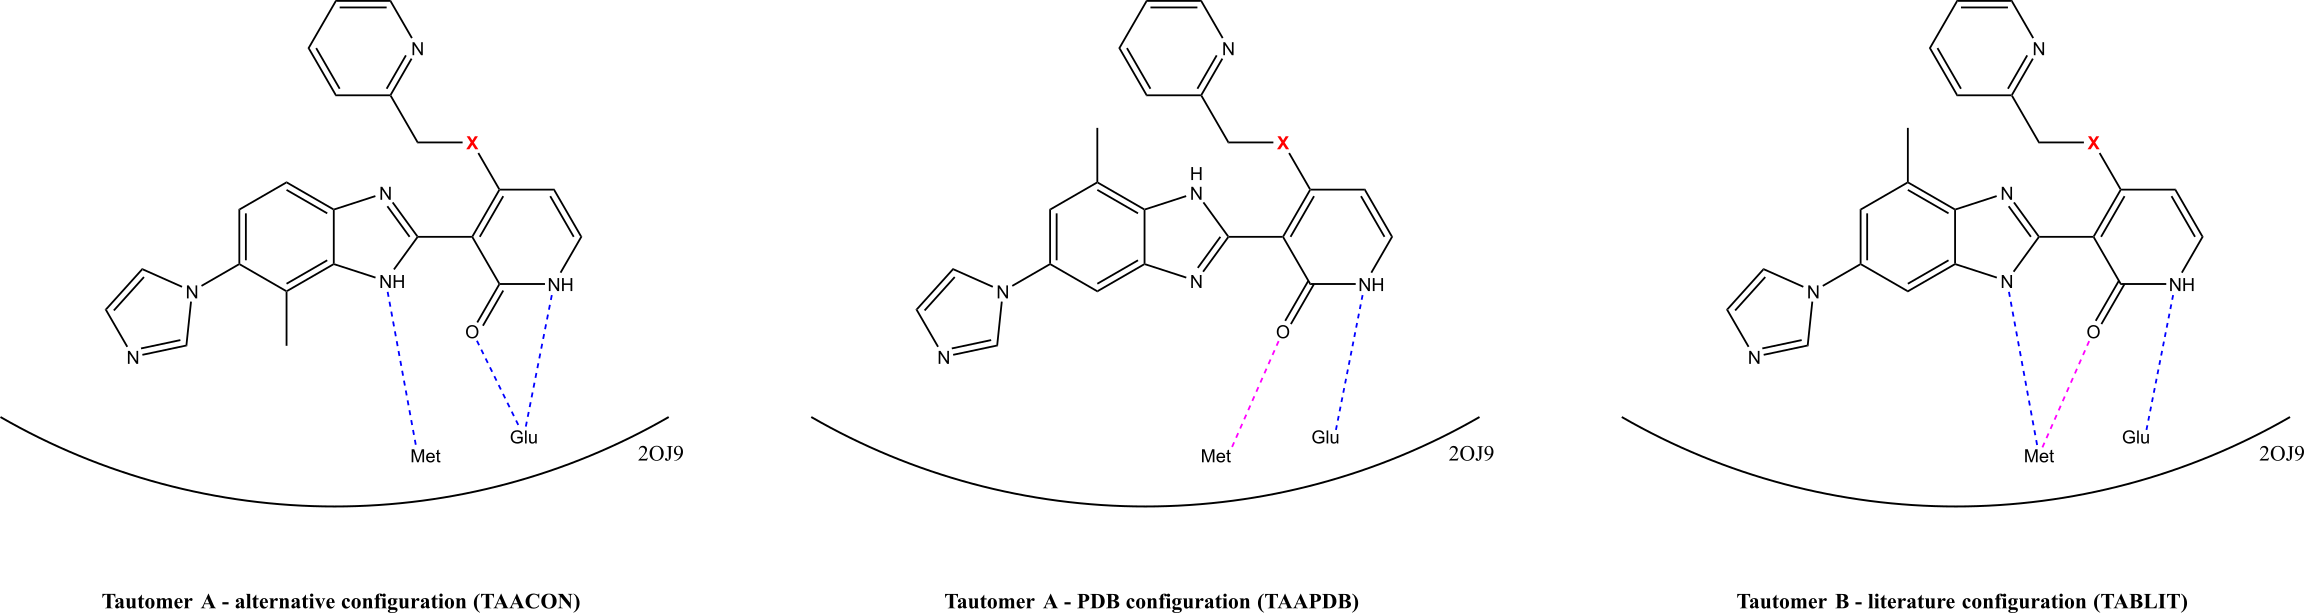
\includegraphics{2oj9_strucs.png}
    \caption[The varieties of BMI bound to 2OJ9] {The varieties of BMI bound to 2OJ9. The red X is substituted with the appropriated functional group of the modification observed, with standard BMI possessing an NH group in its place. Dashed bonds indicate likely interactions with protein amino acids, with violet bonds indicating deviations to TAACON}
    
\end{figure}

2OJ9\footnote{https://www.rcsb.org/structure/2oj9} is a complex of the IGF-1-R insulin growth factor with 3-[5-(1H-imidazol-1-yl)-7-methyl-1H-benzimidazol-2-yl]-4-[(pyridin-2-ylmethyl)amino]pyridin-2(1H)-one (BMI) as inhibitor, first discovered by Velaparthi et. al. in 2007 \cite{velaparthi_discovery_2007}. IGF-1-R has continued to gather medical attention, especially due to its likely role in tumor promulgation \cite{chiu_disruption_2018}. Velaparthi et. al. discuss the impact a variety of substitute operations in BMI have on inhibition. A number of these proposed substitutes, using their numeric identifiers were used for simulations: 24 - NH was used as the baseline comparison due to its high reported binding affinity, with 25 - sulfur and 26 - oxygen also simulated (refer to Fig. \ref{fig:strucs_2oj9} for placement).

All 2OJ9 derivatives were prepared using the standard procedure outlined in section \ref{sec:simulations}.
\subsubsection{VIM-2 with zinc ligands}

VIM-2 is a Carbapenem-Hydrolyzing Metallo-$\beta$-Lactamase, responsible for a subtype of bacterial drug resistance.\cite{Poirel2000Apr}. ZN148, ZN223, and their derivatives are specific zinc ligands first presented by Samuelsen et al.\cite{Samuelsen2020Jun}. These ligands are designed to inhibit Vim2 activity and suppress its drug-resistant activity, thus providing a treatment vector for strains containing it. 

To prepare the structures for use in transformato, protonation states were determined by use of ProToss\cite{Lippert2009Dec,Bietz2014Dec} and manual observation, after which ligand and protein were solvated using CHARMM-GUI's solvation builder, including patching of the C-Terminus. As certain binding modes require the presence of an OH$^-$ group nearby, but CHARMM-GUI's solvation builder is unable to process the system with it, a roundabout way was chosen where a separate .crd file for the OH group was created and patched in after solvation using \texttt{macha}\cite{twotoneblue2022May}. As this also complicated HMR, Hydrogen Mass Repartitioning was accomplished using \texttt{parmed}\cite{Shirts2016Sep}. Afterwards, use in \texttt{Transformato} continued as normal.

Tests included a total of five different ZN* - ligands as denoted in Figure \ref{fig:strucs_vim2}. Nomenclature follows the original used by Samuelsen \cite{Samuelsen2020Jun}.

\begin{figure}\label{fig:strucs_vim2}
    \centering
    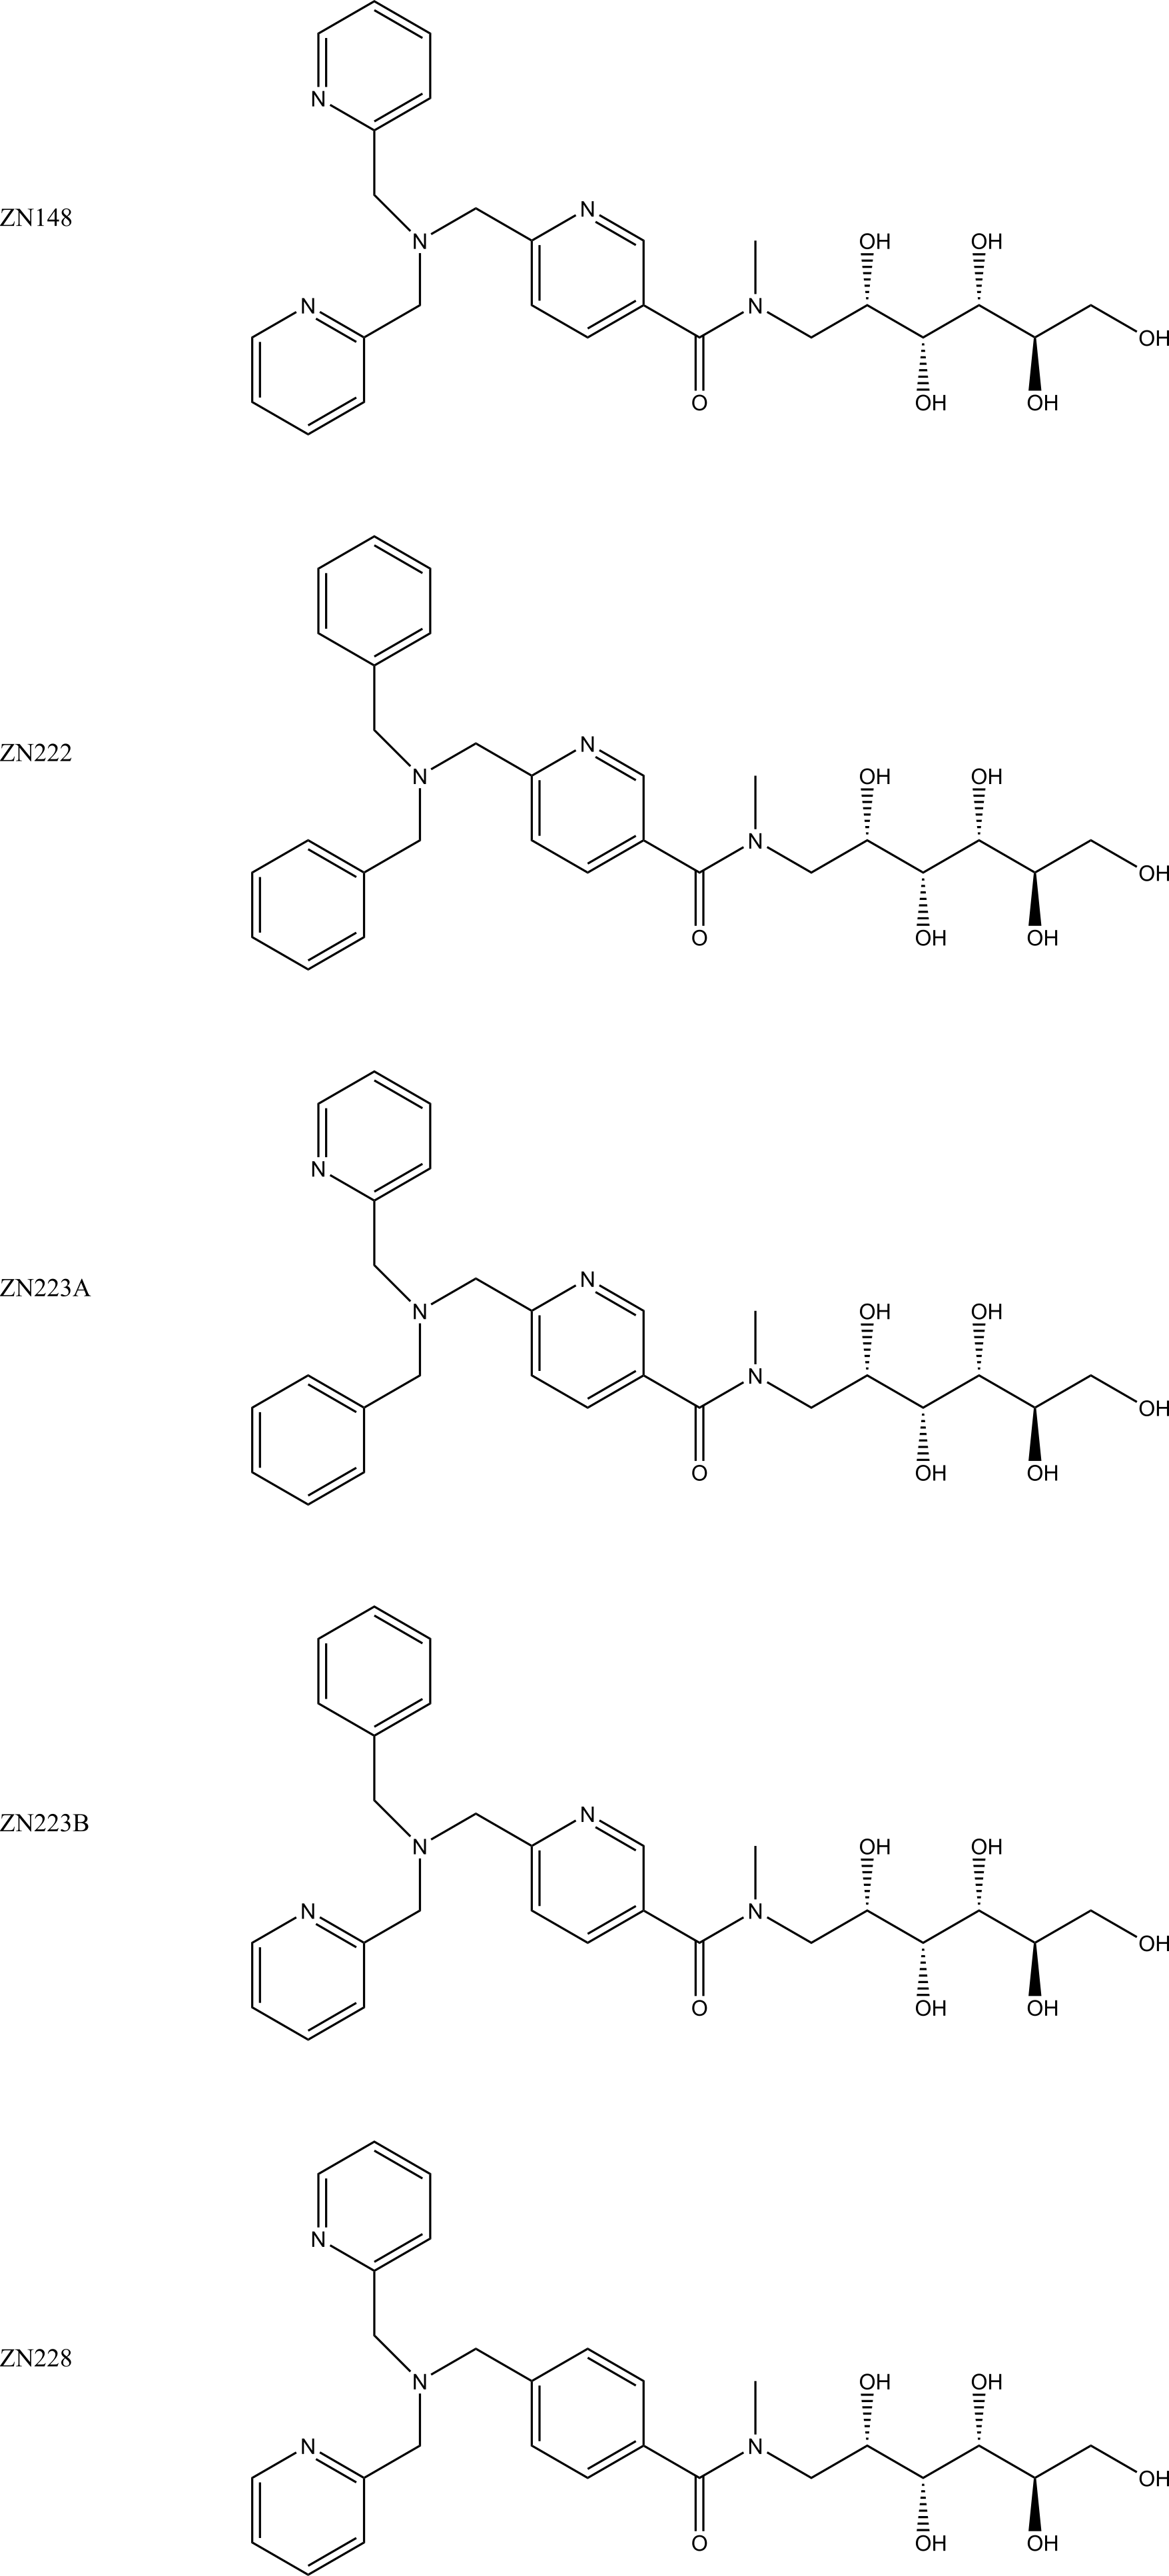
\includegraphics[width=0.4\textwidth]{vim2strucs.png}
    \caption[The various ZN* - ligands bound to VIM2] {The various ZN* - ligands tested against VIM-2.}
    
\end{figure}
\subsection{Binding site dynamics simulations}

Initial efforts were focused on workable implementations of restraints into an openMM system. To that effect, a number of simulations were conducted using 2OJ9. These did not utilize \texttt{Transformato} but rather a variety of dedicated testing scripts. Trajectories were analyzed with regard to the relative distance allowed by various restraints and parameters, the effects of their applications on the complex' total potential energy and its root mean square deviation of atomic position (RMSD), a method to measure positional changes of non-hydrogen protein atoms against the original structure \cite{yusuf_alternative_2008}.

For 2OJ9 derivatives, relative distances were measured according to the likely interaction partners depending on the structure used (refer to Fig. \ref{fig:strucs_2oj9}. Limited simulations were also undertaken using VIM-2. Here, the distance between the nitrogen in the heterocycles to the next acidic hydrogen was measured. 
\subsection{\texttt{Transformato} RBFE calculations}
\begin{figure}[h]\label{fig:CCnotEq}
    \centering
    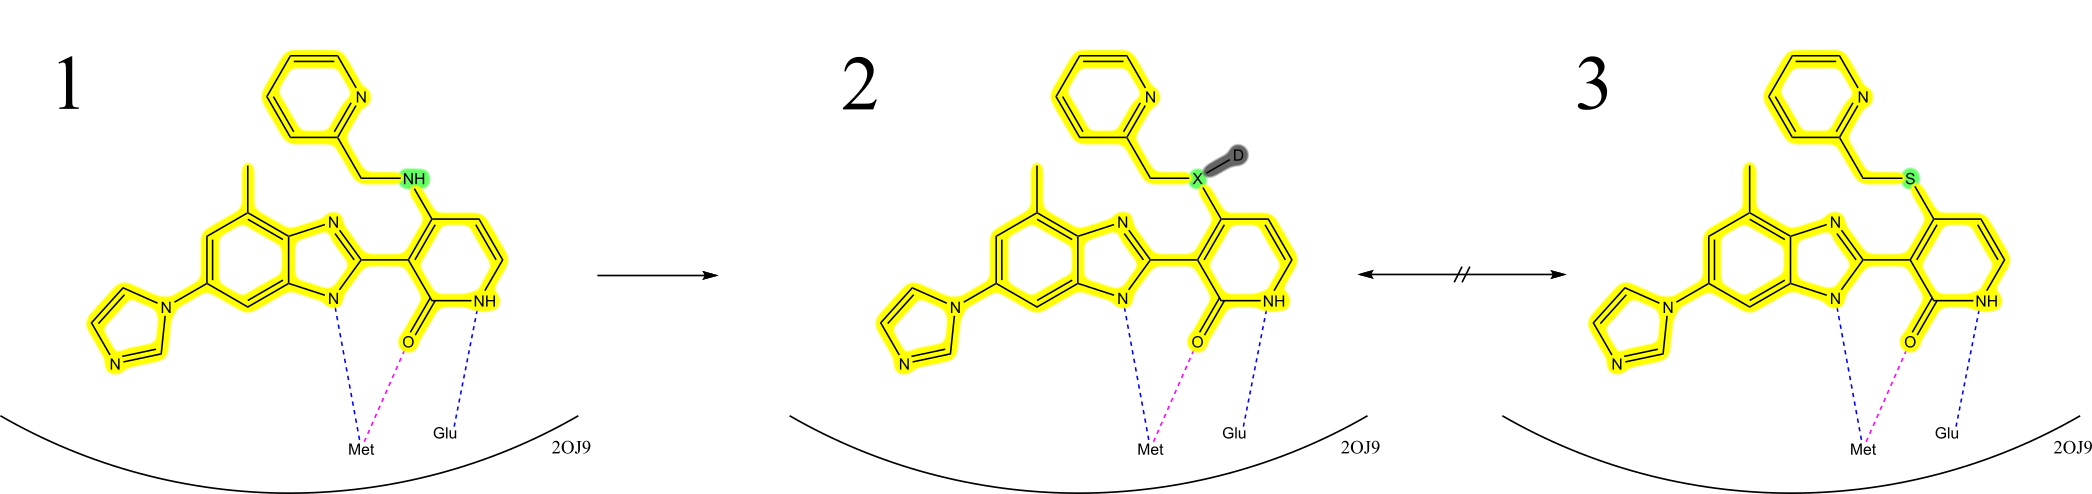
\includegraphics[width=1\textwidth]{CCnotEq.png}
    \caption[Schematic Display of mutation occurring for 2OJ9 TABLIT 24 to the common core with TABLIT 25.]{Schematic Display of mutation occurring for 2OJ9 TABLIT 24 to the common core with TABLIT 25. Yellow: Common Core. Green: Objects that will be mutated. Grey: The dummy region resulting from the superfluous hydrogen. As apparent, the common core (2) resulting from mutation of (1) is not exactly equivalent to the unmated structure (3)}
    
\end{figure}
Here, the focus lay primarily on showing whether the introduction had a significant effect on calculated RBFE. No RSFE simulations were conducted. To facilitate this, 2OJ9 and VIM-2 systems were restrained using a variety of parameters and compared to equal-conditioned unrestrained simulations. Three replicates were used for each set of parameters. As the simulations were resource-intensive, simulations were only conducted one-sided, meaning that only one endstate was mutated into the common core, with the other endstate being chosen in such a way that it was structurally identical to the common core. However, due to differences arising from charge compensation in the terminal junction (see Fig. \ref{fig:CCnotEq}) this means that despite the identical structure this does not supplant a full two-sided simulation. As such, all results are qualitative rather than quantitative.



\chapter{Results}

\section{Binding site dynamics simulations}


\section{\texttt{Transformato} RBFE calculations}

\newpage

\chapter{Discussion}

\section{Comparison to experimental results}
\section{Limitations of the current approach and future possibilities }
\chapter{Annex}
\section{Definitions}
As far as possible, equations in this thesis are notated and styled as in the Alchemistry Wiki maintained by Shirts and Chodera \cite{shirts_alchemistrywiki_nodate}. The symbols and notations used resolve as follows:
\begin{center}
    

\begin{tabular}{ | m{3cm} | m{10cm}| }
\hline
$Q$ & the partition function of the ensemble \\
\hline
$k_B$ & Boltzmann's constant\\
\hline
$T$ & Temperature \\
\hline
$P$ & Pressure \\
\hline
$V$ & (Box) Volume\\
\hline
$U$ & Sum of internal energy in a MD simulation, both potential and kinetic energies\\
\hline
$N$ & Number of particles in the system\\
\hline
$\beta$ & Substitute for $(k_B T)^{-1}$ by convention \\
\hline
$\Gamma$ & Phase Space Volume \\
\hline
$\lambda$ & the \emph{alchemical variable} or \emph{coupling parameter}. Used to describe the progress of a transformation along the alchemical path\\
\hline
$K$ & The \emph{state variable}, describing all conditions and parameters of the thermodynamic system\\
\hline
$k$ & A specific state found in $K$\\
\hline
$u$ & The \emph{reduced potential} $u=\beta(U+PV-\sum{\mu N_i}) $. For NPT ensembles, $\sum{\mu N_i} = 0$\\
\hline
\end{tabular}
\end{center}
\listoffigures

\listoftables

\printbibliography[title={References}]%heading=subbibnumbered,
\end{document}